\documentclass[xcolor=dvipsnames]{beamer}
\usepackage[bars]{beamerthemetree} % Beamer theme v 2.2

\usepackage{graphicx,subfigure,url}
\usepackage[]{lmodern}
\usepackage[]{inconsolata}
\usepackage[]{mathpazo}
\usepackage[]{booktabs}
\usepackage[]{caption}

\usepackage[utf8]{inputenc}
\usepackage[T1]{fontenc}

\renewcommand\familydefault{\rmdefault}
\usepackage[frenchle]{babel}

% example themes
% \usetheme{Goettingen}
% \usecolortheme{seahorse}
% \usecolortheme{rose}

% put page numbers
% \setbeamertemplate{footline}[frame number]{}
% remove navigation symbols
% \setbeamertemplate{navigation symbols}{}

\title{Résultats préliminaires}
\author{Samuel BARRETO}

\begin{document}

\frame[plain]{\titlepage}

\begin{frame}[plain]{Premiers résultats}
	\tableofcontents
\end{frame}

\section{Observations globables}
\label{sec:observ-glob}

\subsection{Comptages}

\begin{frame}{Observations globables}
  \begin{columns}
    \begin{column}{.5\textwidth}
      \scriptsize
      \begin{table}[htbp]
        \centering
        
\begin{tabular}{cc}
\toprule
mutant & count\\
\midrule
strong & 83\\
weak & 87\\
\bottomrule
\end{tabular}

        \caption*{Nombres de séquences par manip}
      \end{table}

      \begin{table}[htbp]
        \centering
        
\begin{tabular}{cc}
\toprule
mutant & count\\
\midrule
strong & 1236\\
weak & 1192\\
\bottomrule
\end{tabular}

        \caption*{Nombre de SNP par manip}
      \end{table}
      
    \end{column}
    
    \begin{column}{.5\textwidth}
      \begin{table}[htbp]
        \centering
        
\begin{tabular}{cc}
\toprule
Type de mutation & nombre\\
\midrule
SW & 1188\\
WS & 1237\\
WW & 3\\
\bottomrule
\end{tabular}

        \caption*{Nombre de mutation par type}
      \end{table}
      
    \end{column}
  \end{columns}

  
\end{frame}

\subsection{Qualité}
\begin{frame}{Qualité des séquences}
  \begin{columns}[t]
    \column{.5\textwidth}
    \centering
    \begin{figure}
      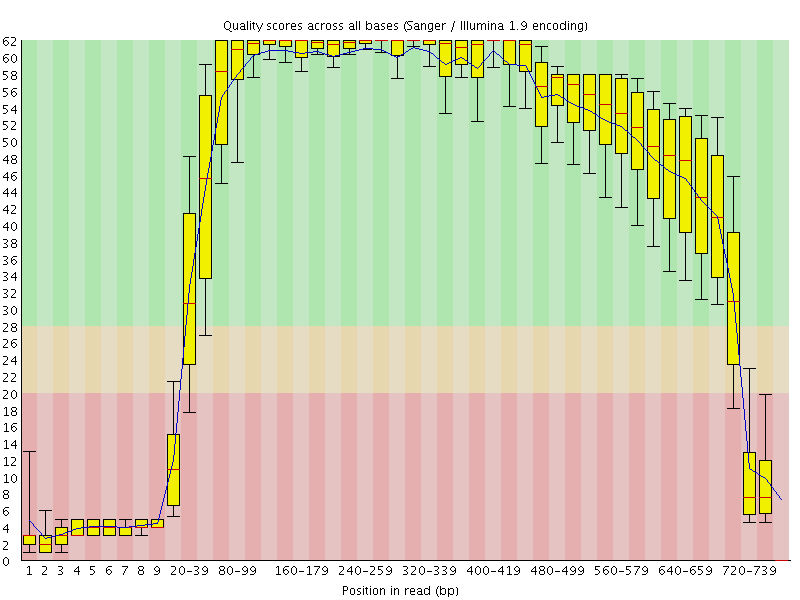
\includegraphics[width=\linewidth]{../per_base_quality_fastqc_untrimmed.png}
      \caption*{Séquences non trimmées}
    \end{figure}
    \column{.5\textwidth}
    \centering
    \begin{figure}[htbp]
      \centering
      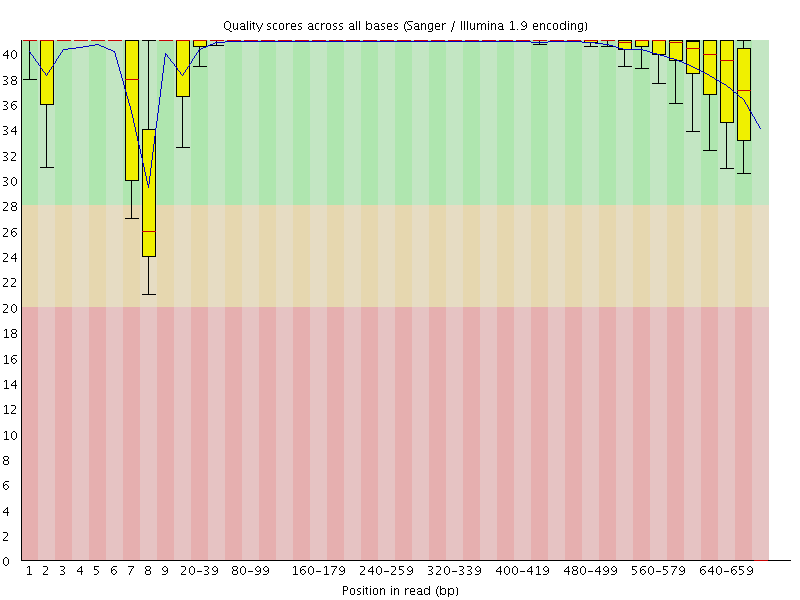
\includegraphics[width=\linewidth]{../per_base_quality_fastqc_trimmed.png}
      \caption*{Séquences trimmées}
    \end{figure}
  \end{columns}
\end{frame}


\section{Distribution des SNP}
\subsection{Globale}

\begin{frame}{Distribution globale des SNP}
  \begin{figure}[htbp]
    \centering
    \includegraphics[width=0.8\linewidth]{../snp_distribution.pdf}
    \caption*{Quantité de SNP par position et par manip}
  \end{figure}

\end{frame}

\subsection{Position terminale de switch}
\begin{frame}{Position terminale de switch}
  \begin{figure}[htbp]
    \centering
    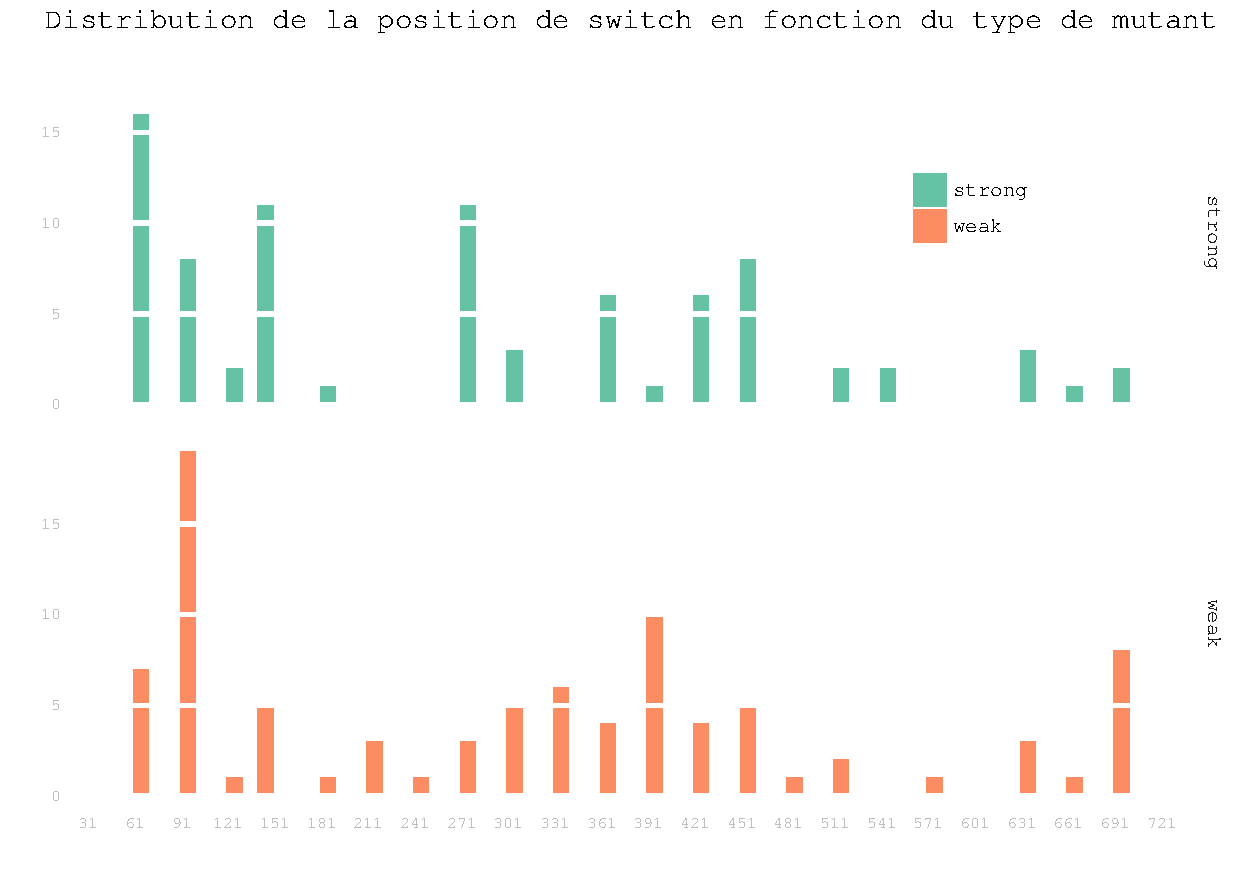
\includegraphics[width=0.8\linewidth]{../switch_distrib.pdf}
  \end{figure}

\end{frame}



\section{Polymorphisme}
\subsection{Spectrogrammes}

\begin{frame}{Sur les spectrogrammes}
  \begin{figure}[htbp]
    \centering
    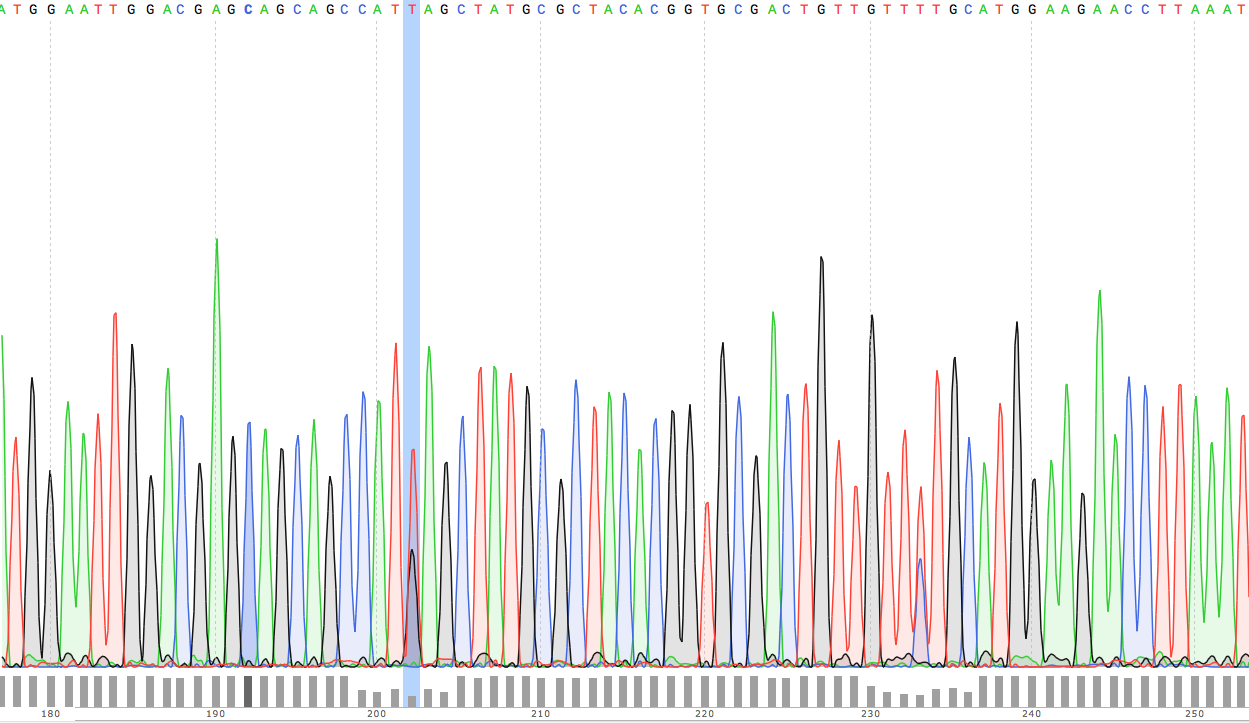
\includegraphics[width=\linewidth]{../weak_spectro.png}
    \caption*{Pour la manip Weak}
  \end{figure}

\end{frame}

\begin{frame}{Sur les spectrogrammes}
  \begin{figure}[htbp]
    \centering
    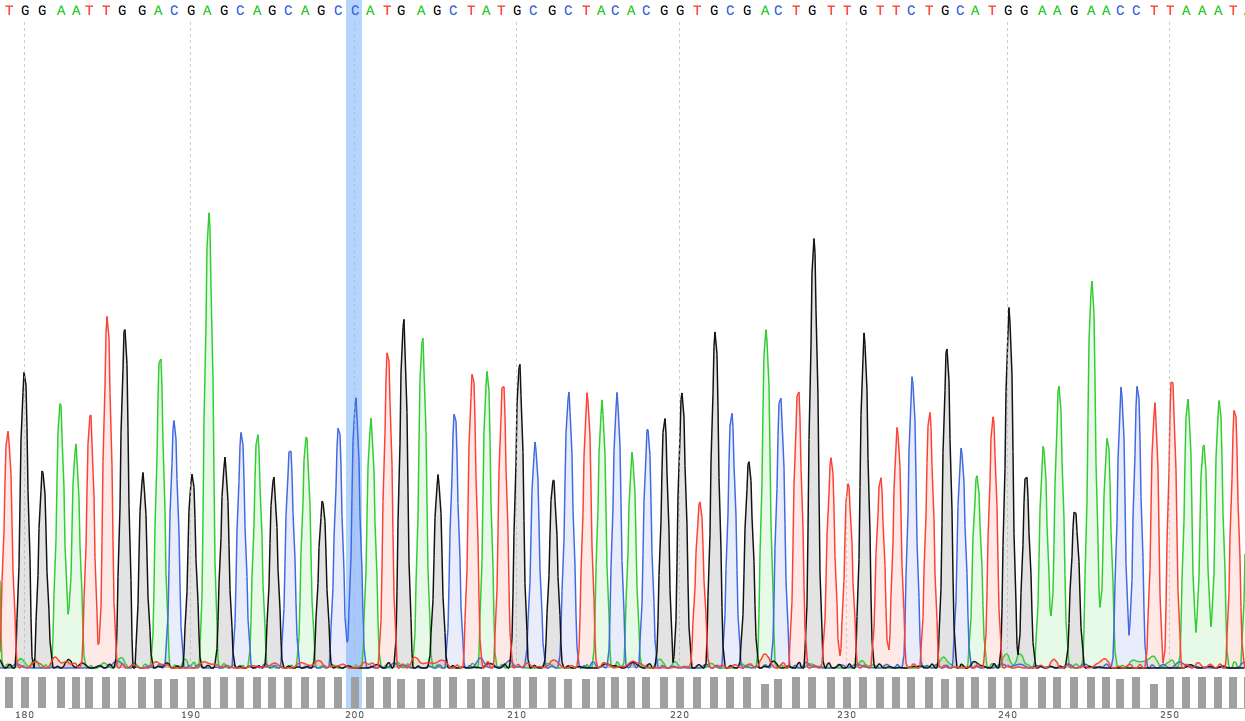
\includegraphics[width=\linewidth]{../strong_spectro.png}
    \caption*{Pour la manip Strong}
  \end{figure}

\end{frame}

\subsection{Globalement}
\label{subsec:globaemnet}

\begin{frame}{Le polymorphisme est weak spécifique}
 \begin{figure}[htbp]
   \centering
   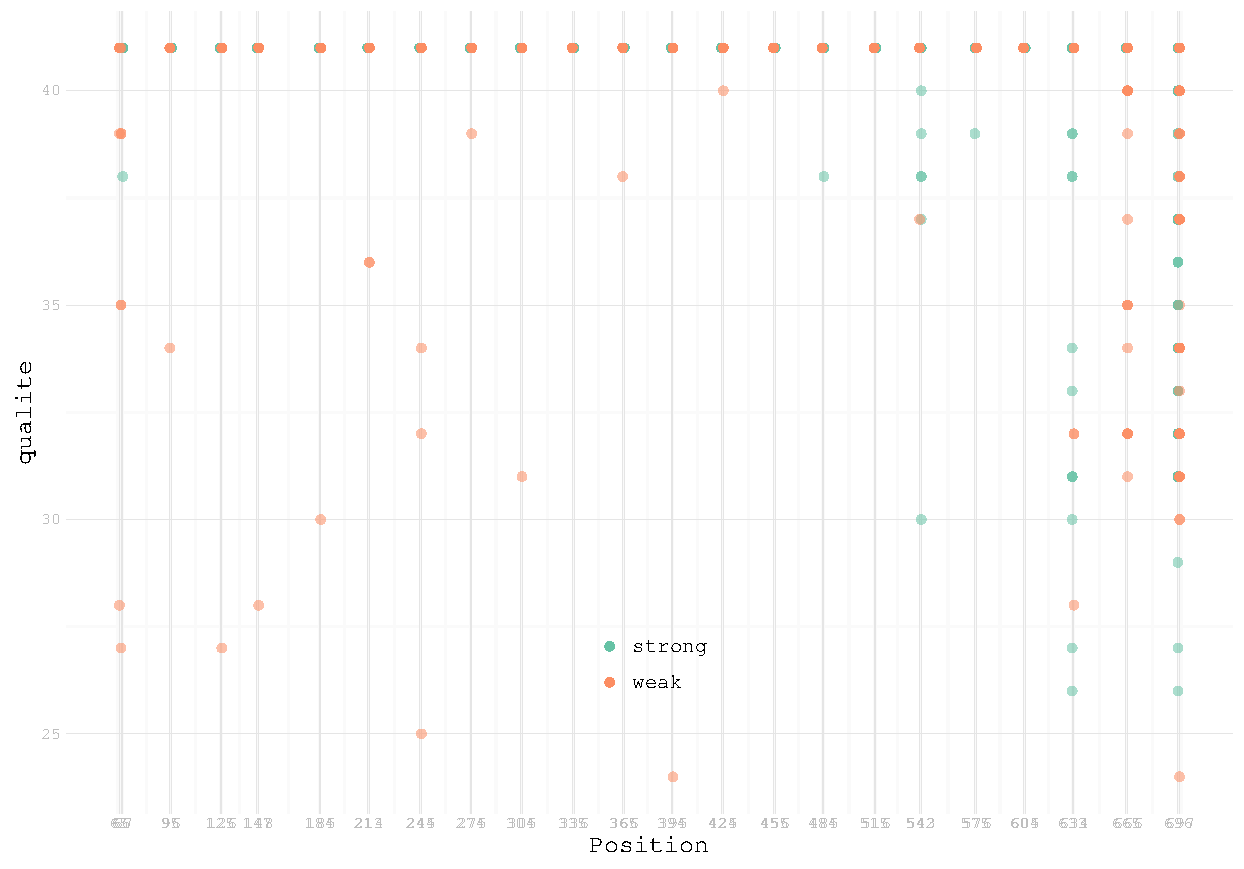
\includegraphics[width=0.8\linewidth]{../qualite_distrib.pdf}
 \end{figure}
 
\end{frame}

\begin{frame}{Le polymorphisme est weak spécifique}
  \begin{columns}
    \begin{column}{.7\textwidth}
      \begin{figure}[htbp]
        \centering
        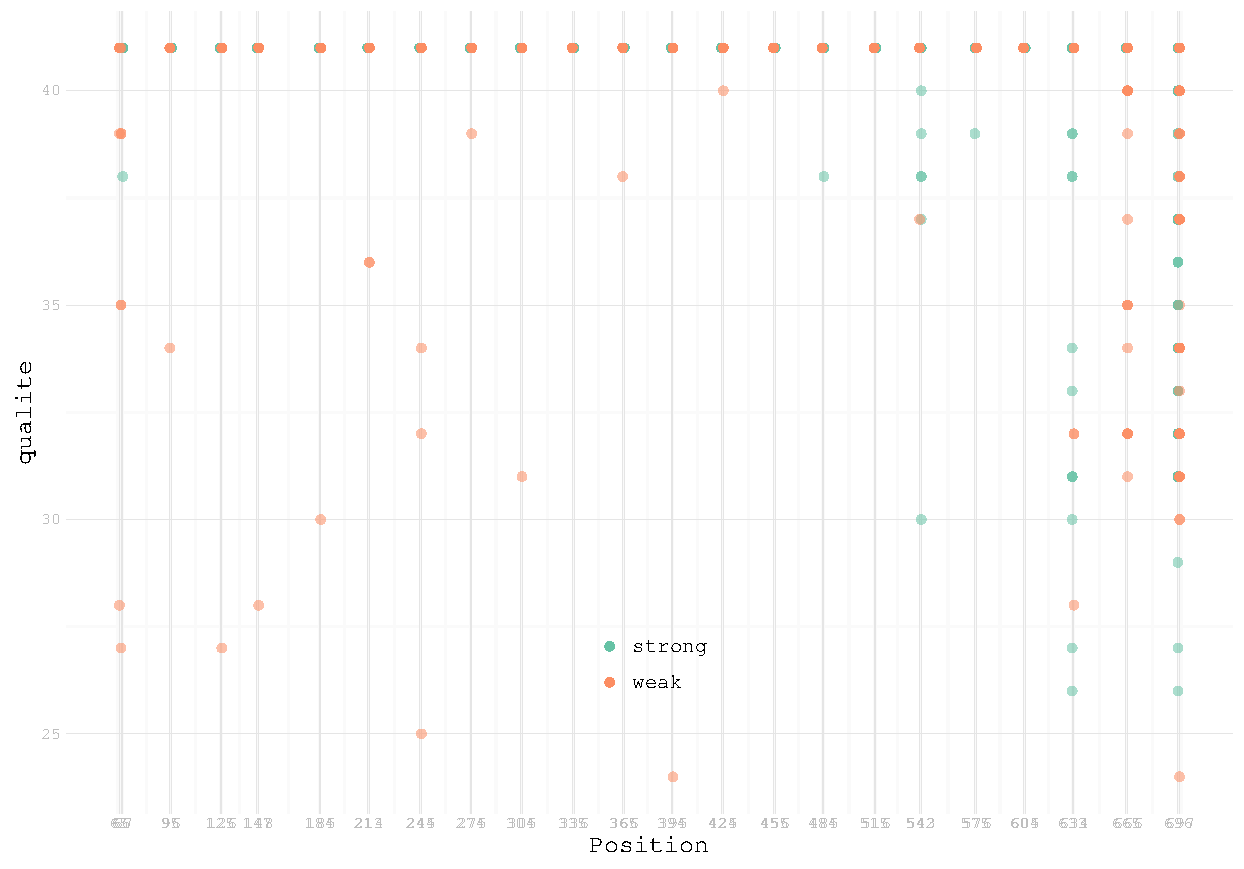
\includegraphics[width=0.8\linewidth]{../qualite_distrib.pdf}
      \end{figure}
      
    \end{column}
    
    \begin{column}{.3\textwidth}
      \tiny
      \ttfamily
      \begin{table}[htbp]
        \centering
        
\begin{tabular}{lr}
\toprule
mutant & count\\
\midrule
strong & 8\\
weak & 21\\
\bottomrule
\end{tabular}

        \caption*{\tiny Nombre de SNP aux positions attendues dans la région <
          600 de qualité inférieure à
          40. Il n'y a pas de néomutations de qualité inférieure à 40}
      \end{table}
      \begin{table}[htbp]
        \ttfamily
        \centering
        \begin{tabular}{cl}
          \toprule
          mutant & count\\
          \midrule
          Strong &  0.008629989\\
          Weak & 0.02320442\\
          \bottomrule
        \end{tabular}
        \caption*{\tiny En fréquence}
      \end{table}
    \end{column}
  \end{columns}
\end{frame}

\section{Néo-mutations}

\begin{frame}{Les néomutations sont W $\rightarrow$ S}
  \begin{center}
    % latex table generated in R 3.2.2 by xtable 1.8-0 package
% Thu Dec  3 18:39:36 2015
\begin{table}[ht]
\centering
\begin{tabular}{cc}
  \hline
Type de Substitution & Nombre \\ 
  \hline
SW &   3 \\ 
  WS &  12 \\ 
  WW &   3 \\ 
   \hline
\end{tabular}
\end{table}

  \end{center}

  \begin{figure}
    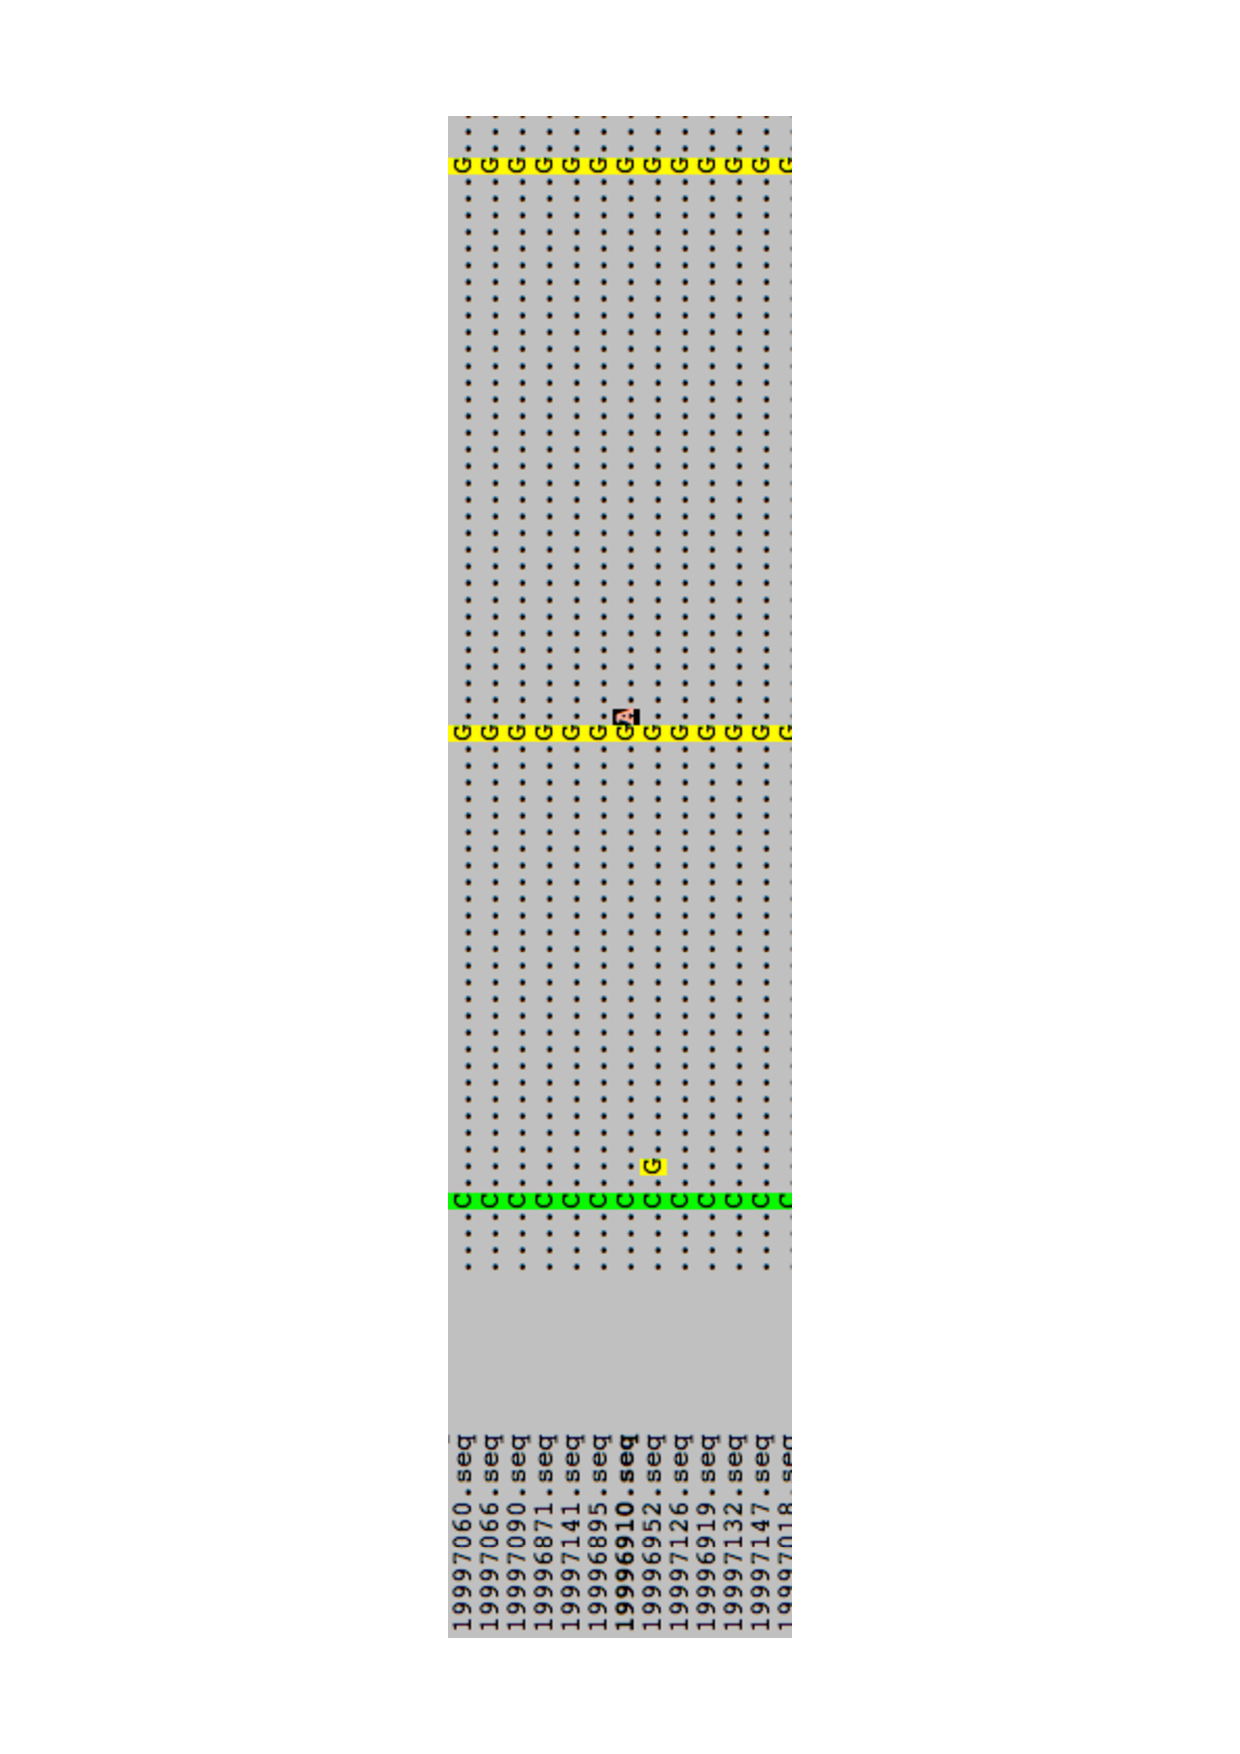
\includegraphics[width=\linewidth]{../inattendu.png}
    \caption*{Il faut faire attention aux mutations de ce genre : c'est une
      mutation W dans la manip strong, à une position attendue de la manip Weak.}
  \end{figure}
\end{frame}

\begin{frame}{Distribution des néomutations}
  \begin{figure}[htbp]
    \centering
    \includegraphics[width=0.8\linewidth]{../bgc_en_action.pdf}
  \end{figure}
\end{frame}

\begin{frame}{Dans la conversion tract ?}
  \begin{center}
  
\begin{tabular}{l|r}
\hline
inside\_conv & count\\
\hline
non & 2\\
\hline
oui & 16\\
\hline
\end{tabular}

  \end{center}
\end{frame}




\end{document}
